\documentclass{article}
\usepackage{graphicx}
\usepackage{wrapfig}
\usepackage{subcaption}
\usepackage[margin=1in]{geometry}
\usepackage{amsmath} % or simply amstext
\usepackage{amssymb}
\usepackage{siunitx}
\usepackage{booktabs}
\usepackage[export]{adjustbox}
\newcommand{\angstrom}{\textup{\AA}}
\newcommand{\colormap}{jet}  % colorbar to use
\usepackage{cleveref}
\usepackage{booktabs}
\usepackage{gensymb}
\usepackage{float}

\title{Statistical Inference of Transport Mechanisms and Long Time Scale Behavior from Time Series 
       of Solute Trajectories in Nanostructured Membranes.}

\author{Benjamin J. Coscia, Christopher P. Calderon \and Michael R. Shirts} 

\begin{document}

  \graphicspath{{./figures/}}
  \maketitle
  
  % BJC2: I'm not putting a lot of effort into the introduction since I'll only write
  % an abbreviated form for my dissertation. I'll work on the intro after my defense.  

  \section{Introduction}
  
  There is a need for highly selective membranes in order to perform efficient 
  separations of components of complex aqueous streams.
  %MRS2: add some more examples (When you get around to it).
  \begin{itemize}
    \item Organic micropollutants
    \item Desalination and boric acid removal from seawater.
    \item While many researchers focus on membrane permeability, we may be 
    able to reduce costs of commercial nanofiltration and reverse osmosis with
    higher selectivity.~\cite{werber_materials_2016}
  \end{itemize}

%  \noindent Amphiphilic molecules are capable of self-assembling into ordered nanostructures.
%  \begin{itemize}
%    \item 
%  \end{itemize}

  Lyotropic liquid crystals (LLC) are a class of amphiphilic molecules whose ordered phases
  can be cross-linked into mechanically strong membranes capable of highly selective
  separations.
  \begin{itemize}
    \item The shape of the LLC monomers and water content dictates the ordered phase 
    that they form. There are two phases of particular interest for membrane applications.
  	\item H\textsubscript{II} phase lyotropic liquid crystals are characterized by 
  	hexagonally packed, straight, pores while the Q\textsubscript{I} phase consists of
  	a tortuous network of 3D interconnected pores. 
  	\item In both cases the pores are uniform in size with radii on the order of 1 nm
    %MRS2: is it really a molecular weight cutoff?
    %BJC2: is molecular size better? Obviously there are other factors like shape, but I don't want to get into that
  	giving them a very strict molecular size cut-off.
	\item Additionally, they have the potential to disrupt conventional membrane separation
	techniques by being selective based not only on size and charge, but on chemical
	functionality as well.
	\item Their pores are lined with LLC monomer functional groups which can potentially
	be designed to interact with solutes in a chemically-specific manner
  \end{itemize}

  There are limits to what we can learn from experiment about LLC membrane design.
  \begin{itemize}
    \item Experimental observables like permeability and selectivity allow us to speculate
    about the molecular origins of separation processes.
    %MRS2: not quite sure what you mean below?
    \item This drives an empirical design approach which can potentially neglect key
    interactions which influence selectivity.
    \item LLC membranes have been shown to exhibit selectivities which cannot be fully 
    explained by relatively simple macroscopic models. 
  \end{itemize}
  
  Molecular Dynamics (MD) simulations can give us mechanistic insights with atomistic 
  resolution so that we can intelligently design new membranes for solute-specific 
  separations.
  \begin{itemize}
    \item In our previous work, we built a detailed atomistic model which we used
    to understand the nanoscopic structure of an LLC Membrane.~\cite{coscia_understanding_2019}
    \item We also used the model in order to gain a qualitative understanding of 
    trapping mechanisms which lead to subdiffusive transport behavior.~\cite{coscia_chemically_2019}
  \end{itemize}

  Unfortunately, the timescales that we can simulate with MD are insufficient to be
  able to make well-converged predictions of macroscopic transport properties 
  traditionally used to characterize membranes in the lab.
  \begin{itemize}
    %MRS2: would be good to get this next point into the first line of a paragraph, since it's quite important. 
    \item However, if we use descriptive stochastic models that can capture solute
    dynamics, then we could project long timescale behavior in addition to gaining
    a deeper understanding of solute behavior on short timescales.
  \end{itemize}
  
  In our previous work, we designed two different approaches which used
  solute time series in order to parameterize stochastic models that could be used
  to project transport on much longer timescales.
  \begin{itemize}
  	\item In our first approach we modeled solute trajectories as subordinated fractional
  	Brownian and L\'evy motion, called the anomalous diffusion (AD) model. 
  	\item We generated solute trajectories by generating a series
  	of anti-correlated hops separated by random periods of entrapment drawn from a 
  	power law distribution.
  	\item Our second approach treated solute motion as a Markov state model with
  	state-dependent dynamics, called the Markov state-dependent dynamical model (MSDDM).
  	\item We parameterized the state transition probabilities between
  	each of eight discrete states as well as the solute dynamics within each of these
  	states. We generated stochastic trajectory realizations by drawing a state
  	sequence based on the transition probability matrix and incorporating the state dynamics
  	while solutes were trapped in each state.
%  	\item Both models had moderate success reproducing the mean squared displacements (MSDs)
%  	exhibited by solutes in our MD simulations.
  \end{itemize}
  
  Although both models had reasonable success at predicting solute mean squared 
  displacements (MSDs) on MD simulation timescales, they had shortcomings.
  \begin{itemize}
  	\item The MSDDM failed to reproduce the hopping and trapping behavior that
  	characterizes solute center-of-mass trajectories in our MD simulations.
  	\item The AD model did not suffer this qualitative shortcoming, but the 
  	persistent curvature of the predicted MSD curves suggested that the model
  	might underestimate MSDs on long timescales. 
  	\item The formulation of both models required careful examination and
  	characterization of the interactions and dynamics exhibit by MD trajectories 
  	which required considerable human effort.
  \end{itemize}
  
  % BJC: Not sure whether to call it the infinite hidden markov model or hierarchical dirichlet process hidden markov model
  % The former is definitely simpler.
  % MRS: True.  I would probably see which is used more in the literature. 
  % BJC1: going with IHMM. HDPHMM seems to mostly be used by Emily Fox
  In this work, we apply the infinite hidden Markov Model (IHMM), a modeling
  approach that is agnostic to the source of time series data, in order to 
  automatically detect and infer the parameters of an unknown number of latent
  autoregressive (AR) modes present in solute center-of-mass time series.
  \begin{itemize}
  	\item In addition to AR parameters for each state, the IHMM estimates the
  	state transition probability matrix.
  	\item The model helps simultaneously uncover underlying transport mechanisms which
  	give rise to dynamical behavior and project that behavior on longer timescales so
  	that we can estimate macroscopic transport observables.
  \end{itemize}
  
  We use the parameters of the states identified by the IHMM in order to infer 
  dominant solute-membrane interactions and transport mechanisms.
  \begin{itemize}
    \item We compare the inferred mechanisms to those which we manually
    identified in our previous work. 
    %MRS2: don't put the conclusions in the introduction.  Instead, state clearly the questions you will ask and the hypotheses you will test.
   \item Some kind of conclusion here. Did we find more or less states. Any new states/ subdivisions of states?
  \end{itemize}
  
  We can also use the IHMM to generate stochastic trajectory realizations that share
  the same dynamical characteristics as solute trajectories observed in our MD 
  simulations. 
  \begin{itemize}
    \item The trajectories are qualitatively similar, showing expected hopping and trapping
    behavior.
    \item They are quantitatively similar in that they reproduce the MSDs measured in MD.
  \end{itemize}

  Finally, we use the stochastic trajectory realizations in order to compute the 
  macroscopic flux of each solute and selectivity of the LLC membranes studied towards
  each solute.
  \begin{itemize}
    %MRS2: shouldn't reach conclusions in intro, just set up questions to be answered (conclusions SHOULD be in abstract).
    \item We relate these macroscopic properties to our nanoscopic model by simulating 
    mean first passage time (MFPT).
    \item Some kind of conclusion. This membrane is selective towards solutes with this
    functionality. 
    \item Does the conclusion agree with our previous work? Any length dependence? (I think not)
  \end{itemize}
    
  \section{Methods}
    
  We ran all MD simulations and energy minimizations using GROMACS 2018. We
  performed all post-simulation trajectory analysis using python scripts which are available
  online at \\ \texttt{https://github.com/shirtsgroup/LLC\_Membranes}.

  \subsection{Molecular Dynamics Simulations}
  
  % BJC: Could I just reference previous work here? "MD simulations were run as 
  % described in our previous work..."
  % BJC2: Or I could just say that I'm using the same data from the last paper. See that paper.

  We studied transport of solutes in the H\textsubscript{II} phase using an
  atomistic molecular model of four pores in a monoclinic unit cell with 
  10 \% water by weight. 
  \begin{itemize}
    \item Approximately one third of the water molecules occupy the tail region 
    with the rest near the pore center.
    \item We chose to study the 10 wt \% water system because solutes move 
    significantly faster than in the 5 wt \% system studied previously.
    \item Appropriate stochastic modeling requires that solutes sample the 
    accessible mechanisms with representative probability.%MRS: only possible on the ~1-10 \mu scale with relatively fast solutes.
  \end{itemize}
  
  We chose to study a subset of 4 of the fastest moving solutes from our previous
  work: methanol, acetic acid, urea and ethylene glycol.
  \begin{itemize} 
    \item In addition to exploring membrane structural space the most, these solutes
    have a relatively diverse set of chemical functionality.   
    \item For each solute we created a separate system and to each system we
    added 6 solutes per pore for a total of 24 solutes.
    \item This number of solutes per pore provides a balance of a low 
    degree of interaction between solutes and sufficient amount of data from
    which to generate statistics on the time scales which we simulate.
    \item Further details on the setup and equilibration of these systems can
    be found in our previous work.\cite{coscia_chemically_2019}
  \end{itemize}
  
  \noindent We extended the 1 $\mu$s simulations of our previous work to 5 $\mu$s in order
  to collect ample data.
  \begin{itemize}
    \item We simulated the system with a time step of 2 fs at a pressure of 1 bar
    and 300 K controlled by the Parinello-Rahman barostat and the v-rescale thermostat
    respectively.
    \item We recorded frames every 0.5 ns
  \end{itemize}

  \subsection{The Infinite State Hidden Markov Model}\label{method:IHMM}
  %BJC: There is a fair amount of detail here just so I could understand better by writing it out
  
  Hidden Markov models (HMMs) are a useful and widely used technique
  for modeling sequences of observations where the probability of the next observation
  in a sequence depends, at least in, part on a previous unobserved, latent or hidden, state.~\cite{beal_infinite_2002}
  %MRS2: it can depend on other things, but ALSO depends on the latent state.
  %BJC2: added 'at least in part
  \begin{itemize}
    \item In the context of our simulations, the observations correspond to 
    the center of mass coordinates of the solutes versus time, and the states
    correspond to the dynamical behavior which give rise to those types
    of observations.
    \item Unfortunately, standard HMMs require the number of hidden states to be known
    a priori.
    \item One can partially overcome this by testing a range of numbers of 
    hidden states and determining which is the best representation of the
    data.
  \end{itemize}
  
  %BJC: I'm not sure how much of this I should include. This is pretty much 
  % a reproduction of Fox et al's explanation: https://ieeexplore.ieee.org/abstract/document/5563110
  % and it doesn't do a great job
  The infinite-state HMM overcomes this drawback by placing a hierarchical
  Dirichlet process (HDP) prior on the transition probabilities.
  \begin{itemize}
    \item Using some base probability distribution, H, a Dirichlet process 
    (DP) generates distributions over a countably infinite number of 
    probability measures:
    \begin{equation}
      G_0 = \sum_{k=1}^{\infty} \beta_k \delta_{\theta_k} ~~ \theta_k \sim H, \beta \sim GEM(\gamma)
    \end{equation}
    where the $\theta_k$ are values drawn from the base distribution and the
    weights $\beta_k$ come from a stick-breaking process parameterized by the concentration 
    parameter $\gamma$ (equivalently referred to as GEM($\gamma$)). 
    \item The concentration parameter expresses one's confidence in H relative to the posterior 
    and is closely related to the number of data observations.
    \item Each row, $G_j$, of the transition matrix is produced by drawing from a DP specified 
    using the $\beta$ vector as a discrete base distribution and a separate concentration
    parameter, $\alpha$.
    \begin{equation}
      G_j = \sum_{k=1}^{\infty} \pi_{jk} \delta_{\theta_k} ~~ \pi_j \sim DP(\alpha, \beta)
    \end{equation}
    \item This hierarchical specification ensures that the transition probabilities in 
    each row share the same support points \{$\theta_1$, ..., $\theta_k$\}.
    \item Once the model has converged only a finite number of states will have significant
    sampling.
  \end{itemize}
  
  %BJC: I do need to include this
  \noindent We describe the dynamics of each state using a first order vector autoregressive
   (VAR(1)) model. 
  \begin{itemize}
  	\item In general, a VAR($r$) process is characterized by a vector of observations in a time series 
  	that are linearly dependent on $r$ previous values of the time series vector:
  	\begin{equation}
  	\mathbf{y}_t = \mathbf{c} + \sum_{i=1}^r A_i\mathbf{y}_{t-i} + \mathbf{e}_t~~~~\mathbf{e}_t \sim \mathcal{N}(0, \Sigma)
  	\label{eqn:var}
  	\end{equation}
  	Previous observations are weighted by coefficient matrices $A_i$. The VAR($r$) 
  	process is further characterized by a shift in the mean of each dimension by the
  	vector $\mathbf{c}$ and a white noise term $\mathbf{e}_t$.~\cite{hamilton_time_1994}
        %MRS2: mean is zero in Z, is it necessarily in R (I realize we've talked about this before, but wanted to get the clarification in text)
    %BJC2: The mean I'm talking about below is different than you are describing above.
    % The multivariate Gausian noise is coming from N(0, \Sigma)
  	\item We assumed $\mathbf{e}_t$ to be multivariate Gaussian noise, with mean zero and
  	covariance, $\Sigma$.
  	\item We limited our analysis to an autoregressive order of $r=1$.
  	\item We used a conjugate matrix-normal inverse-Wishart prior on parameters
  	$A$ and $\Sigma$ and a conjugate Gaussian prior on $\mathbf{c}$ in order to analytically
  	draw from the posterior.~\cite{fox_nonparametric_2009}
  \end{itemize}   
  
  %Based on the algorithms developed by Fox et al.~\cite{fox_sticky_2007}, 
  Using the IHMM framework, we estimated the most likely number and sequence of hidden states
  while simultaneously estimating VAR(1) parameters for each state and the overall 
  state transition probability matrix, $T$.
  \begin{itemize}
    \item We created a python implementation of this process which we heavily adapted from
    the MATLAB code of Fox et al.~\cite{fox_sticky_2007} 
    \item Parameter estimation is iterative. Therefore, we looked for convergence 
    as shown in SI.
    \item We refer the interested reader to much more extensive descriptions of 
    this process and its implementation. 
    ~\cite{beal_infinite_2002,teh_hierarchical_2006,van_gael_beam_2008,fox_nonparametric_2009,fox_bayesian_2010}
  \end{itemize}
  
  There are many ways one can apply the IHMM algorithm to timeseries data. 
  \begin{itemize}
    \item We begin by trying to identify as many distinct states as possible
    in each solute trajectory and then take advantage of the system's cylindrical
    symmetry in order to cluster the parameter sets into an interpretable number
    of states.
    \item Having a large number of states gives more reliable clustering results.
%    \item We believe the subsequent procedure is best suited for our data
%    because it can clearly distinguish different dynamical behavior, it takes
%    advantage of the system's cylindrical symmetry and represents distinct
%    dynamics in an interpretable number of states.
  \end{itemize}
  
  %BJC2: this is hard to word clearly. Maybe a small figure would help
  We first applied the IHMM algorithm to the 3D solute center-of-mass coordinate 
  trajectories transformed relative to the closest pore center.
  \begin{itemize}
    \item We tracked the solute's motion along the pore axis with center-of-mass
    $z$ coordinate.
    \item Using the nearest pore center as the origin, we represented the radial 
    distance of each solute's center-of-mass from the pore center in 2 dimensions,
    $x$ and $y$.
    \item By using 2 dimensions, rather than a single radial dimension, we
    increase the likelihood of finding more states since a single radial
    mean can be represented by an infinite number of $x$ and $y$ coordinate combinations.
  \end{itemize}
  
  \begin{figure}
  \centering
  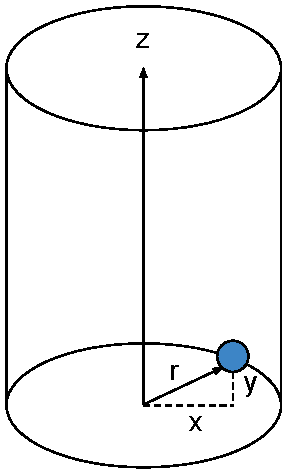
\includegraphics[width=0.2\textwidth]{cartesian_cylinder.pdf}
  \caption{Using the nearest pore center as the origin, we represented the solute's
  location along the pore axis in terms of the $z$ coordinates and their radial distance
  from the pore centers in 2 dimensions, $x$ and $y$.}\label{fig:cartesian_cylinder}
  \end{figure}
  
  We applied the IHMM to each of the 24 solute trajectories independently.
  \begin{itemize}
    \item Although the IHMM is capable of identifying an infinite number of states, 
    a Dirichlet Process tends to exhibit a ``rich get richer" effect, favoring
    a fewer number of states.
    \item By applying the algorithm to each trajectory independently we reduce
    the possibility of lumping together multiple similar states which we
    would prefer to stay separated before clustering.
%    \item From a practical implementation standpoint, the algorithm is written
%    such that we must put a cap on the maximum number of states. We chose to 
%    allow up to 100 states for each trajectory although the algorithm typically
%    finds within the range of 5-15 states. 
    % BJC2: There will probably be a figure telling the number of states for 
    % each trajectory.
  \end{itemize}
  
  The states predicted by the IHMM are heavily influenced by the Gaussian prior
  placed on $c$ in Equation~\ref{eqn:var}.
  \begin{itemize}
    \item The $A$ and $\mathbf{e}_t$ matrices do not vary over a wide range, so
    the final parameters were relatively insensitive to the priors.
    \item In order to maximally automate the IHMM procedure, we attempted to
    parameterize the prior on $c$ in an intelligent way.
    \item The prior parameters should be chosen such that the means of 
    each state lie within a region of reasonable probability of the prior (see
    Figure~\ref{fig:prior_guesses}).
    \item In each dimension, we defined the prior mean to be halfway between the 
    maximum and minimum of each trajectory dimension. 
    \item We defined the maximum and minimum to be 2 standard deviations from
    the mean in order to parameterize the variance in each dimension.
    \item Although this approach has worked quite well for the data in this work,
    it is important to check the results to determine whether further adjustments
    to the prior might be needed.
    \item In the Supporting Information, we show the result of a parameterization
    where the prior parameters of $c$ were poorly chosen.
  \end{itemize}
  
  %BJC2: I think it would be useful to continue using this trajectory to illustrate 
  % the parameterization process. It might be bunch of plots stacked on each other.
  \begin{figure}
  \centering
  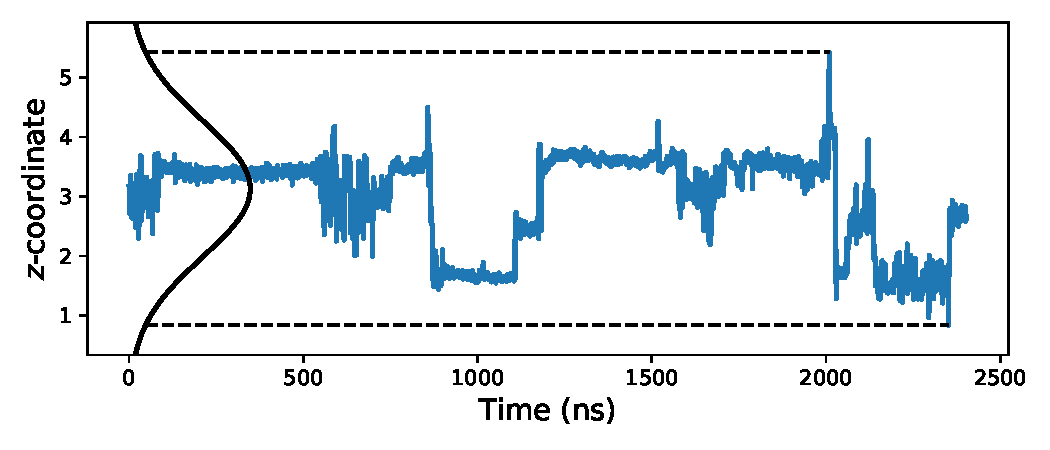
\includegraphics[width=\textwidth]{prior_guesses.pdf}
  \caption{The parameters of the prior on $c$ (black line) should be chosen such
  that the means of each state identified in the trajectory (blue line) lie within
  regions of the prior with reasonable probability. We chose the mean of the prior 
  as halfway between the maximum and minimum of each trajectory dimension. We also
  defined the maximum and minimum to be 2 standard deviations from the mean in 
  order to parameterize $\sigma$.}\label{fig:prior_guesses}
  \end{figure}
  
  We ran 2000 iterations of the IHMM procedure in order to arrive at converged 
  state sequence and parameters for each state.
  \begin{itemize}  
    \item Most parameters converged quickly (within 50-100 iterations) while
    others took up to 1000 iterations.
    \item We averaged the parameters from each iteration after the equilibration
    time point.
    \item We detected equilibration of the parameters using the module 
    \texttt{pymbar.timeseries.detect\_equilibration} on the time series of 
    parameter estimates. 
    \item Since all of the parameters are multidimensional, we found the 
    equilibration time point of each component and then used the longest
    equilibration time of all dimensions as the equilibration time point.
  \end{itemize}
  
  % BJC2: It's probably possible to convert to from x, y, z to r, z but
  % I need to figure out the transformation of A. This approach works though.
  We reparameterized the time series, preserving the state sequence, in terms
  of the radial and axial coordinates ($r$, $z$) because the mean in $r$ is 
  a useful clustering variable.
  \begin{itemize}
    \item It will also be clearer to analyze the final parameter set in
    terms of $r$ rather than $x$ and $y$.
    \item We converted the $x$ and $y$ center-of-mass coordinates to $r$.
    \item In order to keep the same states found by applying the algorithm
    in 3D, we reapplied the IHMM to the cylindrical trajectories, only allowing
    inference on the VAR(1) parameters with a fixed state sequence. 
  \end{itemize} 
  
  We clustered like parameter sets in order to reduce the state space to
  a more easily interpretable size.
  \begin{itemize}
   \item For each solute studied, we identified between 200-300 independent sets of
   parameters. % BJC2: just a guess for now
   \item Many of these states exhibit very similar dynamical behavior except their
   mean levels are different, especially in the axial direction where solutes could
   get trapped along a broad and continuous range of $z$ coordinates.
   \item Since we do not know the number of states with shared dynamical behavior
   beforehand, we used a non-parametric Bayesian Gaussian mixture model in order
   to group them. % cite scikit-learn  
   \item This is necessary for us to perform any kind of mechanistic speculation.
  \end{itemize}   
 
  We clustered based on 5 variables: the radial means of each state, the two
  eigenvalues of $A$ and the two eigenvalues of $e_t$.
  \begin{itemize}
   \item Unfortunately, the number of independent parameter sets is too low for
   clustering in higher dimensions. 
   \item Ideally, we could use all of the entries of $A$ and $e_t$ in addition to 
   the radial means.
   \item It would not be helpful to use the means in the $z$ direction because solutes
   are essentially unbound in that direction, while there tends to be radially
   dependent behavior as shown in our previous work.~\cite{coscia_chemically_2019}  % cite new paper too.
  \end{itemize}

  We remapped the state sequence based on the clustered assignments and
  generated a state transition probability matrix, $T$.
  \begin{itemize}
   \item The IHMM algorithm also produces an estimate of $T$, but since we 
   fixed the state sequence, we decided to explicitly calculate $T$ by 
   counting the number of transitions between states.
  \end{itemize}  
  
  We obtained clustered $\mathbf{c}$ vectors based on the means of 
  $\mathbf{c}$ belonging to the same cluster.
  \begin{itemize}
   \item We only care about the $r$ component of $c$ because solute
   trajectories are not boudn in the $z$ direction.
  \end{itemize}
  
  We used the IHMM algorithm in order to infer $A$ and $e_t$ of the 
  clustered states.
  \begin{itemize}
   %BJC2: I'm unsure of the precise reasoning here.
   \item We could not simply take the mean of the clustered 
   $A$ and $e_t$ parameters because it is not clear that this is a linear 
   operation for this problem. 
   \item To circumvent this problem, we modified the ($r$, $z$) solute
   trajectories so that they had a mean of zero, leaving only the 
   fluctations. 
   \item We did this by subtracting the maximum likelihood estimate
   of the $\mathbf{c}$ vector from each same-state segement of the unclustered
   trajectory.   
   \item We used the IHMM algorithm on modified this modified trajectory to infer
   the clustered state parameters by fixing the clustered state sequence. 
  \end{itemize}
  
  Finally, we generated stochastic trajectory realizations by drawing state sequences 
  based on the rows of $T$.
  \begin{itemize}
    \item While in a given state, we simulated motion according to the VAR(1)
    parameterization of that state.
    \item We set the unconditional mean of each state based on the position 
    before the state transition occurred.
  \end{itemize} 
  
  \subsection{Estimating Flux and Selectivity}
  %BJC: can make this discussion somewhat short since it's already in previous paper. 
  % Should probably just hit all the main equations quickly.
  
  \noindent We calculate first passage times by propagating stochastic trajectories until they
  reach distance $L$. \\
  
  We determine the mean first passage time (MFPT) using the following equation:~\cite{cussler_diffusion:_2009}
  \begin{equation}
  P(t) = -\frac{1}{\sqrt{\pi}}e^{-(L - vt)^2 / (4Dt)}\bigg(-\frac{D(L - vt)}{4(Dt)^{3/2}} - \frac{v}{2\sqrt{Dt}}\bigg)
  \label{eqn:passage_times}
  \end{equation}
  
  \noindent Flux, $J$, is simply 1 / MFPT by the Hill relation.~\cite{hill_free_1989} \\
  
  In our previous work, we showed that, in the absence of convective solute flux, selectivity
  towards solute $i$ versus solute $j$ can be calculated by:  
  \begin{equation}
  S_{ij} = \frac{J_i / \Delta C_i}{J_j / \Delta C_j}
  \label{eqn:selectivity}
  \end{equation}
  where $\Delta C_j$ is the trans-membrane concentration difference.

  \section{Results and Discussion}
  %MRS2: how stable are the results to realizations of the system
  \subsection{Inferring Solute Transport Mechanisms}
  
  Clustering parameters sets results in X distinct dynamical modes.
  \begin{itemize}
    \item In the figure below, we show time series simulations that qualitatively
    illustrate the difference in dynamical behavior between modes.
  \end{itemize}
   
  %BJC1: a figure showing some representative fluctuations in each mode

  \noindent We can relate the identified states back to transport mechanisms.
  \begin{itemize}
  	\item More detailed discussion of identified states
  	\item How size of fluctuations, autoregressive parameters are influenced by trapping mechanisms
  	\item How do these states compare to those identified in our previous work?
  	\item Any new states?
  \end{itemize}
  
  \subsection{Reproducing MD Trajectories and MSDs with the IHMM}
  
  \noindent Trajectory realizations qualitatively match MD simulation trajectories.

  \begin{itemize}
    %MRS2: think about how to quantify the simiilarity of the hopping and trapping behavior.
    \item Look for hopping and trapping behavior
  \end{itemize}
  
  \noindent MSDs generated from stochastic trajectories match those from MD.
  \begin{itemize}
    %MRS2: again, think about the best ways to quantify similar between MD and stochastic trajectories.
  	\item Look at curvature and 1-$\sigma$ confidence intervals
  \end{itemize}
  
  \subsection{Estimating Solute Flux and Selectivity}  
  
  \noindent We can predict macroscopic flux and selectivity.
  \begin{itemize}
  	\item Flux as function of pore length
  	\item Selectivity as function of pore length (if flux scaling is length-dependent)
  \end{itemize}
 
  \section{Conclusion}
  
  \noindent We have shown that the IHMM can be used to parameterize solute time series
  with an unknown number of latent dynamical modes. \\
  
  \noindent We can use the IHMM to help identify mechanisms by relating the latent
  states to observed solute behavior. \\
  
  \noindent We can use the IHMM to predict macroscopic transport properties. \\
  
  %MRS2: below probably doesn't need to be stated?
  \noindent The IHMM is not limited to the H\textsubscript{II} phase.
  
  \section*{Supporting Information}

  Detailed explanations and expansions upon the results and procedures mentioned in
  the main text are described in the Supporting Information. This information is
  available free of charge via the Internet at http://pubs.acs.org.

  \section*{Acknowledgements}

  %MRS2: add GAANN and PRF here to cover bases.
  This work was supported in part by the ACS Petroleum Research Fund
  grant \#59814-ND7 and the Graduate Assistance in Areas of National Need (GAANN) 
  fellowship which is funded by the U.S. Department of Education. 
  Molecular simulations were performed using the Extreme Science and
  Engineering Discovery Environment (XSEDE), which is supported by National
  Science Foundation grant number ACI-1548562. Specifically, it used the Bridges
  system, which is supported by NSF award number ACI-1445606, at the Pittsburgh
  Supercomputing Center (PSC). This work also utilized the RMACC Summit supercomputer,
  which is supported by the National Science Foundation (awards ACI-1532235 and
  ACI-1532236), the University of Colorado Boulder, and Colorado State
  University. The Summit supercomputer is a joint effort of the University of
  Colorado Boulder and Colorado State University.

  \clearpage

  \bibliographystyle{ieeetr}
  \bibliography{hdphmm}

  %\newpage

  %\section*{TOC Graphic}

\end{document}
